\section{Kommunikation}
Wie im Kapitel \ref{sec:architektur} beschrieben, besteht unsere Anwendung aus drei Komponenten, die untereinander kommunizieren müssen. Das Smartphone spricht auf der einen Seite mit dem Web-Service zur Berechnung des Models, auf dem die Lokalisierung beruht. Auf der anderen Seite sendet es Daten, wie z.B. eine Notiz, und Steuerbefehle an die Smartwatch, um z.B. Bluetooth-Scans zu starten oder zu stoppen. Umgekehrt sendet die Smartwatch Daten an das Smartphone, z.B. die Ergebnisse eines Scans. Die verschiedenen Kommunikationswege und ihre Nutzung werden im Folgenden näher beschrieben.

\subsection{Zwischen Smartphone und Web-Service}

Zur Kommunikation mit dem Web-Service wird eine einfache HTTP-Schnittstelle verwendet.
Der Web-Service erstellt aus den Messungen ein Modell zur Raumerkennung. Dazu
werden die Messungen im CSV-Format gesendet. Das Modell wird als JSON-Objekt
übertragen.

\subsubsection{Datenformate}
TODO: Beispiel für CSV \\
TODO: Beispiel für Modell


\subsubsection{UTF-8}
Bei der Übertragung der UTF-8 Daten aus Android heraus gab es unerwartete Probleme.
Die ersten Tests waren erfolgreich, bis wir ein größeres Datenvolumen erreicht haben.
Da der Web-Service UTF-8 kodierte Daten erwartet, haben wir die Methode \texttt{writeUTF}
der Klasse \texttt{DataOutputStream}
\footnote{\url{https://developer.android.com/reference/java/io/DataOutputStream.html}} 
verwendet. Diese Methode hat allerdings eine Beschränkung auf 64 KB an kodierten Daten.
Also haben wir versucht die Daten in Blöcken von maximal 64 KB zu übertragen. Allerdings
fügt die Methode bei jedem Aufruf einen BOM (Byte-Order-Marker) ein, was dazu führt,
dass die gesendeten Daten kein korrektes UTF-8 mehr enthalten.
Um das Problem zu lösen, mussten wir die UTF-8-Konvertierung selbst durchführen
und Bytes über den Stream senden.

\subsection{Zwischen Smartphone und Smartwatch}
Die Kommunikation zwischen dem Smartphone und der Smartwatch muss bidirektional sein, um die benötigten Funktionalitäten erfüllen zu können. Die Schnittstelle PhoneConnector (Abb. \ref{fig:Klassendiagramme}) beschreibt die Richtung von der Smartwatch zum Smartphone, während die Schnittstelle WatchConnector (Abb. \ref{fig:Klassendiagramme}) die umgekehrte Richtung darstellt.

\begin{figure}[H]
\centering
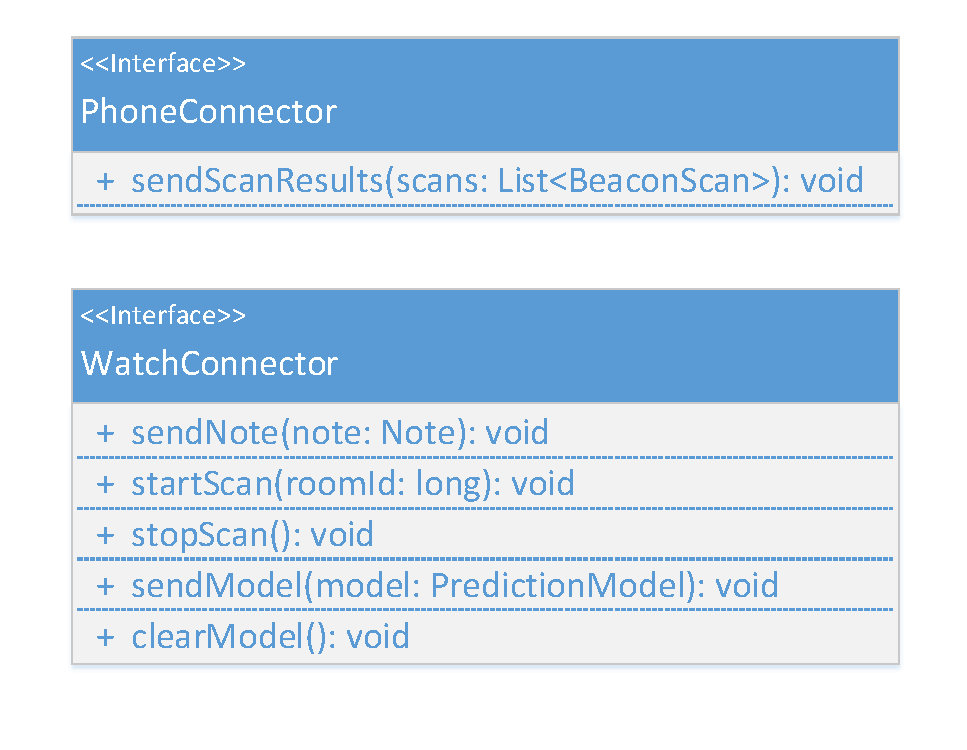
\includegraphics[width=0.5\linewidth]{../Bilder/Klassendiagramme}
\caption{Schnittstellendefinitionen zur Kommunikation zwischen Smartphone und Smartwatch}
\label{fig:Klassendiagramme}
\end{figure}


Kommunikation zwischen einem Android Smartphone und einem Android Wear Gerät findet grundsätzlich über die Wearable Data Layer API\footnote{\url{http://developer.android.com/training/wearables/data-layer/index.html}} statt, die Teil der Google Play Services ist. Die API bietet verschiedene Möglichkeiten der Kommunikation. Wir haben uns in einem ersten Anlauf mit der Synchronisation von sogenannten DataItems beschäftigt. Da diese Synchronisation allerdings nicht sofort nach einer Aktualisierung der Daten stattfindet und somit die Daten nicht sofort bei dem Kommunikationspartner verfügbar sind, implementierten wir die Kommunikation im weiteren Verlauf des Projekts mithilfe von Messages und der dafür vorgesehenen MessageAPI \footnote{\url{http://developer.android.com/training/wearables/data-layer/messages.html}}. Messages stellen eine unidirektionale Kommunikationsmöglichkeit dar. Sie sind definiert über eine Pfadangabe und können beliebige Daten in Form eines Byte-Arrays transportieren. Zum Empfang der Daten dient eine Implementierung des Wearable Listener Services\footnote{\url{https://developers.google.com/android/reference/com/google/android/gms/wearable/WearableListenerService}}.

Um die angesprochen bidirektionale Kommunikation herzustellen, haben wir entsprechend auf jeder Seite der Kommunikationen einen Listener Service implementiert sowie die Möglichkeit geschaffen Messages zu versenden. Am Beispiel der Vermessung zur initialen Erstellung des Models wird die Kommunikation mit Messages im folgenden Sequenzdiagramm (Abb. \ref{fig:SequenzdiagrammScan}) dargestellt.

\begin{figure}[H]
\centering
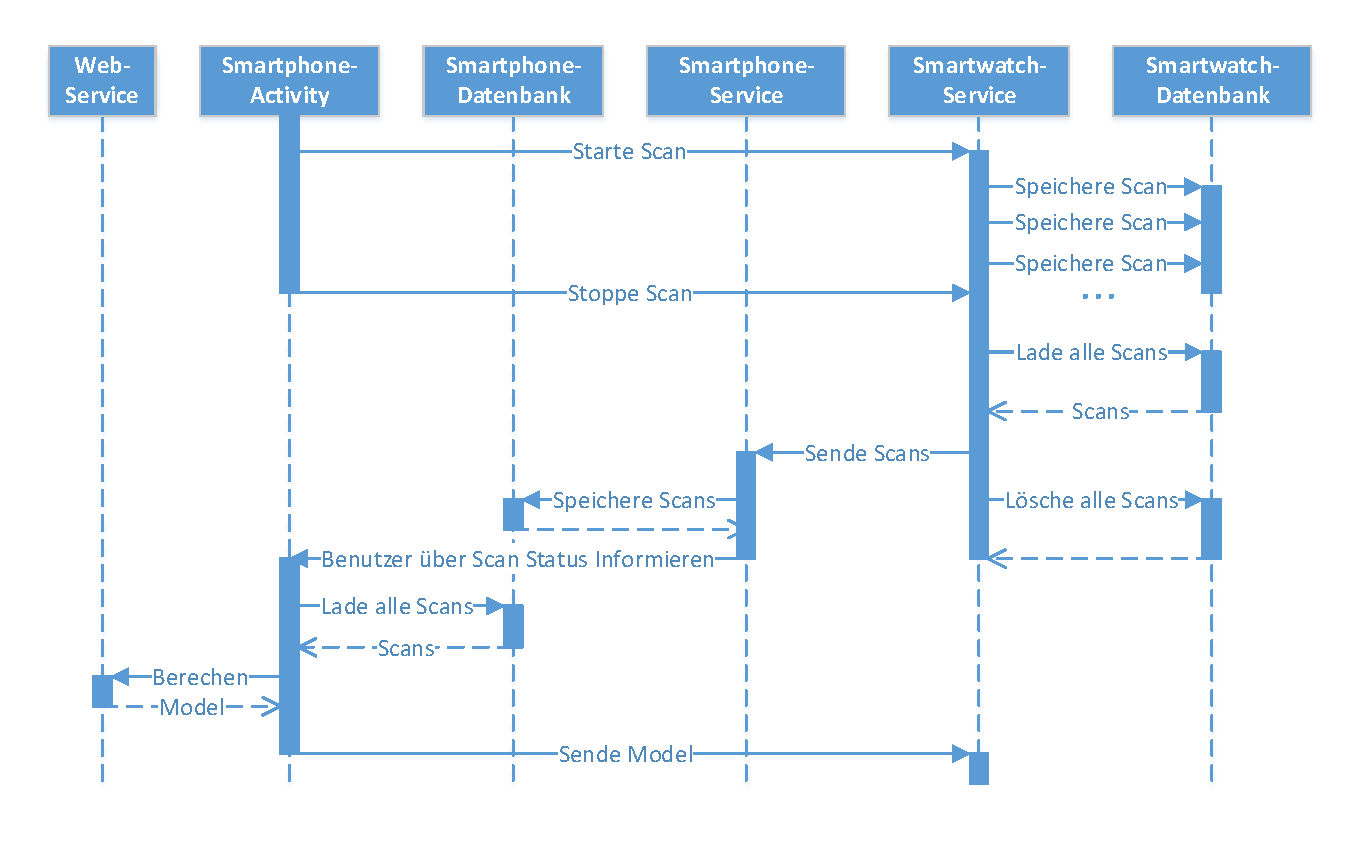
\includegraphics[width=0.9\linewidth]{../Bilder/SequenzdiagrammScan}
\caption{Sequenzdiagramm der Vermessung zur initialen Erstellung des Models}
\label{fig:SequenzdiagrammScan}
\end{figure}

Der Benutzer startet den Ablauf durch die Aktion \textit{Starte Scan} in der Smartphone Activity. Der Smartwatch Service empfängt den Befehl, startet den Scan und speichert die gescannten Werte in der Datenbank. Der Service scannt solange bis der Benutzer mithilfe der Smartphone Activity den \textit{Stoppe Scan} Befehl absetzt. Nachdem der Service das Scannen beendet hat, lädt dieser alle gescannten Werte aus der Datenbank, versendet sie und löscht die Werte aus der Datenbank, um bei Folgescans bei null zu starten. Die versendeten Werte empfängt der Smartphone Service, der diese in der Datenbank des Smartphone speichert und den Benutzer mittels der Smartphone Activity über den abgeschlossenen Scanvorgang informiert. Hat der Benutzer alle Räume vermessen, kann er die Berechnungen des Models anstoßen. Die Smartphone Activity lädt daraufhin alle Scandaten aus der Datenbank und schickt diese zur Berechnung des Models an den Web-Service. Der Web-Service liefert das berechnete Model zurück, welches die Smartphone Activity an den Smartwatch Service versendet, der fortan damit arbeiten kann.

\subsection{Zwischen Service und Activity}
-Service muss Infos weiterreichen
-Service muss Activity starten
-Beispiel Note

